\documentclass{article}
\usepackage{tikz}
\usetikzlibrary{shapes.geometric}
\usetikzlibrary{shapes.arrows}
\usepackage{array}
\begin{document}
\pagestyle{empty}
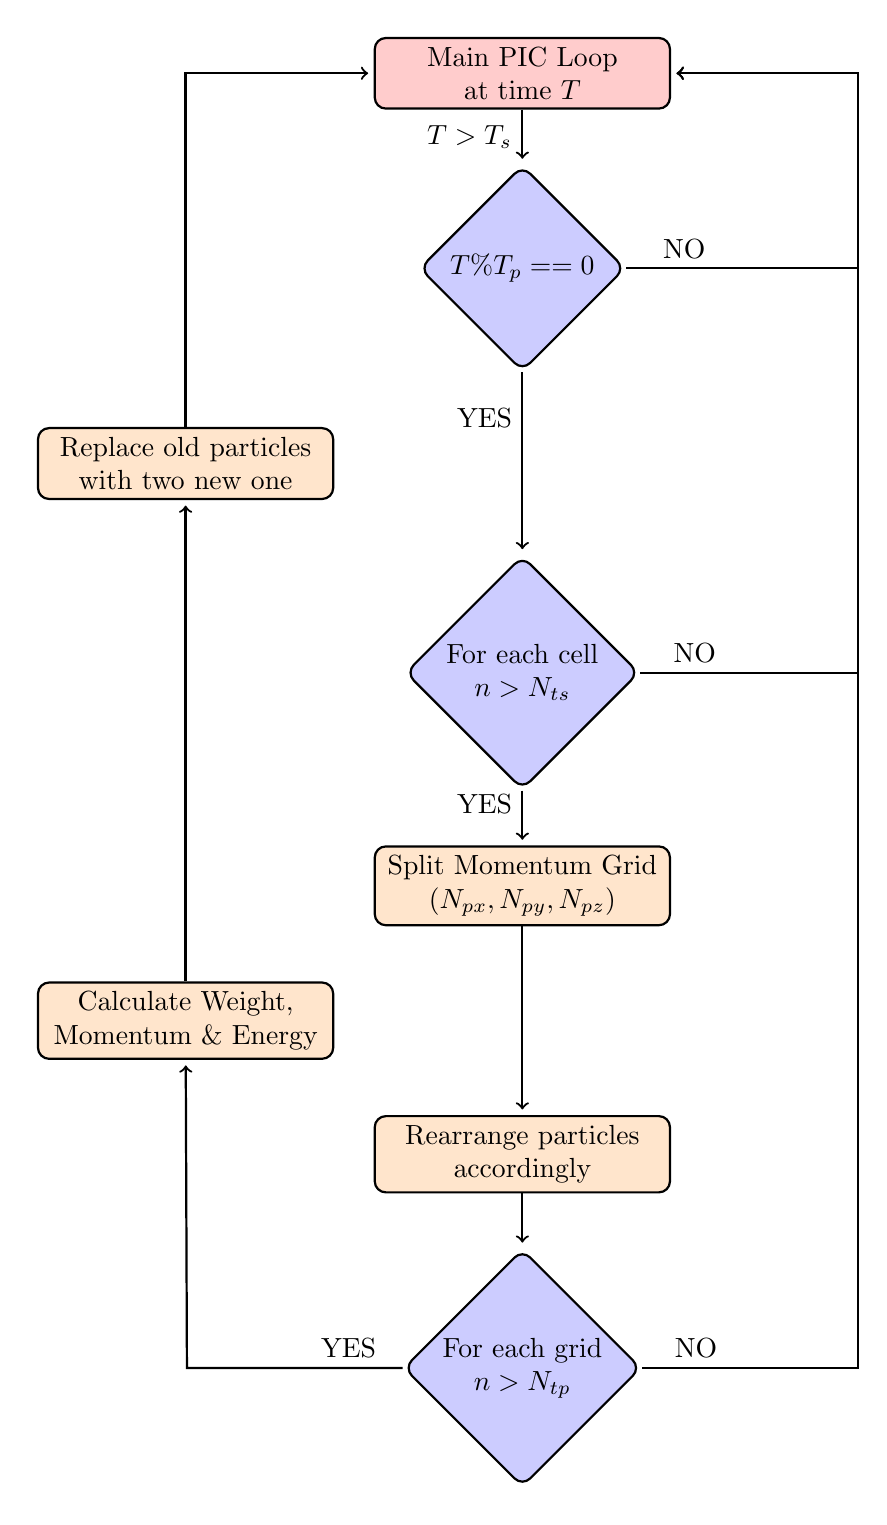
\begin{tikzpicture} [
    auto,
    decision/.style = { diamond, draw=black, thick, fill=blue!20,
                        text width=6em, text badly centered,
                        inner sep=1pt, rounded corners },
    block/.style    = { rectangle, draw=black, thick, 
                        fill=orange!20, text width=10em, text badly centered,
                        rounded corners, minimum height=2em },
    line/.style     = { draw, thick, ->, shorten >=2pt },
    start/.style    = { rectangle, draw=black, thick, 
                        fill=red!20, text width=10em, text badly centered,
                        rounded corners, minimum height=2em },
  ]
  
\matrix [column sep=5mm, row sep=7mm] {
                    & \node [start]    (start) {Main PIC Loop \\ at time $T$};            & \\
                    & \node [decision] (mod)   {$T\%T_p==0$};                              &
                    & \node(null2){};                                                     & \\
                      \node[block](rep){Replace old particles \\ with two new one};
                    & \node(null3){}; & \\
                    & \node [decision] (nts)   {For each cell \\ $n>N_{ts}$};                & \\  \node(null4){};
                    & \node [block]    (pgrid) {Split Momentum Grid \\ $(N_{px}, N_{py}, N_{pz})$}; & \\
                    \node [block]    (calc)  {Calculate Weight, \\ Momentum \& Energy};
                    & \node(null5){}; & \\
                    & \node [block]    (rearr) {Rearrange particles accordingly};        & \\
                    & \node [decision] (ntp)   {For each grid \\ $n>N_{tp}$}; & \\
  };

\begin{scope} [every path/.style=line]
    \path (start)     --     node [anchor=east] {$T>T_s$} (mod);
    \path (mod)       --     node [anchor=east, near start] {YES}        (nts);
    \path (nts)       --     node [anchor=east, near start] {YES}        (pgrid);
    \path (pgrid)     --                                                 (rearr);
    \path (rearr)     --                                                 (ntp);
    % \path (mod)       --     node [anchor=north, near start] {NO}        (null2);
    % \path (null2)     |-                                                 (start);
    \path (mod)       --++  (4.26,0) node [near start] {NO} |-  (start);
    \path (nts)       --++  (4.26,0) node [near start] {NO} |-  (start);
    \path (ntp)       --++  (4.26,0) node [near start] {NO} |-  (start);
    \path (ntp)       --++  (-4.26,0) node [anchor=south, near start] {YES} -- (calc);
    \path (calc)      --                                          (rep);
    \path (rep)       |-                                        (start);
\end{scope}

\end{tikzpicture}
\end{document}